% ----- CHAPTER 1: INTRODUCTION ----- %

Let $E$ be an elliptic curve over the rational numbers. We can think of $E$ as the set of rational solutions $(x,y)$ to a two-variable cubic equation in the form:
\begin{equation}
E: y^2 = x^3 + Ax + B
\end{equation}
for some integers $A$ and $B$, along with an extra "point at infinity". An important criterion is that the $E$ be a smooth curve; this translates to the requirement that the discriminant $D_E$ of the curve, given by $D_E = -16(4A^3+27B^2)$, is not zero.

One of the natural questions to ask when considering an elliptic curve is "how many rational solutions are there?" It turns out elliptic curves fall in that sweet spot where the answer could be zero, finitely many or infinitely many - and figuring out which is the case is a deeply non-trivial -- and as yet still open -- problem.

The rational solutions on $E$ form an abelian group with a well-defined group operation that can be easily computed. By a theorem of Mordell, the group of rational points on an elliptic curve $E(\mathbb{Q})$ is finitely generated; we can therefore write
\begin{equation}
E(\mathbb{Q}) \approx E_{\text{Tor}}(\Q) \times \mathbb{Z}^r,
\end{equation}
where $E_{\text{Tor}}(\Q)$ is a finite group (called the torsion subgroup of $E$), and $r$ is a non-negative integer, denoted the {\it algebraic rank} of $E$.

Determining the torsion subgroup of $E$ is relatively straightforward. By a celebrated theorem of Mazur, rational elliptic curves have torsion subgroups that are (non-canonically) isomorphic to one of precisely fifteen possibilities: $\mathbb{Z}/n\mathbb{Z}$ for $n = 1$ through $10$, or $\mathbb{Z}/12\mathbb{Z}$, or $\mathbb{Z}/2\mathbb{Z}\oplus \mathbb{Z}/2n\mathbb{Z}$ for $n = 1$ though $4$. However, computing the rank $r$ -- the number of independent rational points of infinite order on $E$ -- is hard, and no unconditional method to do so currently exists. It is towards this end that the work in this dissertation hopes to contribute. \\

Perhaps surprisingly, we can translate the algebraic problem of finding the number of rational solutions on $E$ to an analytic one -- at least conjecturally. The method of doing so is via elliptic curve $L$-functions; these are complex-analytic entire functions that somehow encode a great deal of information about the elliptic curve they describe. Unfortunately, it takes a few steps to define them:

\begin{definition}
Let $p$ be a prime number;
\begin{itemize}
\item Define $N_p(E)$ to be the number of points on the {\it reduced curve} $E$ modulo $p$. That is (excepting the cases $p=2$ or $3$, for which the definition is slightly more complicated), if $E$ has equation $y^2 = x^3 + Ax+B$, then
\begin{equation}
N_p(E) = 1 + \#\set{(\xbar,\ybar) \in \Fp^2 : \;\; \ybar \equiv \xbar^3 + A\xbar + B \;\;(\text{mod }p)},
\end{equation}
where the 1 accounts for the aforementioned point at infinity on $E$ not captured by the above equation.
\item Let $a_p(E) = p+1 - N_p(E)$.
\end{itemize}
\end{definition}
Hasse's Theorem states that $a_p(E)$ is always less that $2\sqrt{p}$ in magnitude for any $p$, and the Sato-Tate conjecure (recently proven by Taylor et al.) states that for a fixed elliptic curve, the $a_p$ values, once suitably normalized, are asymptotically distributed in a semi-circular distribution about zero. In other words, the number of solutions to an elliptic curve equation modulo $p$ is always about $p$, and can never be very far from that value.

\begin{definition}  For prime $p$,
\begin{itemize}
\item Define the {\it local factor} $L_p(E,s)$ to be the function of the complex variable $s$ as follows:
\begin{equation}
L_p(s) = \frac{1}{1-a_p(E)p^{-s} + \epsilon(p)p^{-2s}},
\end{equation}
where $\epsilon(p)$ is 0 if $p$ is a {\it prime of bad reduction}, and 1 otherwise. [For any elliptic curve $E$ there are only a finite number of primes of bad reduction; they are precisely the primes that divide the discriminant $D_E$ of a minimal model of $E$].
\item The {\bf (global) $L$-function $L(E,s)$ attached to $E$} is defined to be the product of all the local $L$-functions, namely
\begin{equation}
L(E,s)  = \prod_{p} L_p(E,s).
\end{equation}
\end{itemize}
\end{definition}
The above representation of $L(E,s)$ is called the Euler product form of the $L$-function. If we multiply out the terms and use power series inversion we can also write $L_E(s)$ as a {\it Dirichlet series}:
\begin{equation}
L(E,s) = \sum_{n=1}^{\infty} a_n(E) n^{-s},
\end{equation}
where for non-prime $n$ the coefficients $a_n$ are defined to be exactly the integers you get when you multiply out the Euler expansion.

If you do some analysis using Hasse's bound on the size of the $a_p(E)$ and their distribution according to Sato-Tate, one can show that the above two series converge absolutely when the real part of $s$ is greater than $\frac{3}{2}$ (see Lemma \ref{lem:ldLe_bound} and Corollary \ref{cor:L_E_abs_convergence}) and diverge when the real part of $s$ is less than $\frac{1}{2}$. However, the modularity theorem of Breuil, Conrad, Diamond, Taylor and Wiles \cite{BCDT-2011} \cite{TaWi-1995} \cite{Wil-1995} states that these elliptic curve $L$-functions can actually be analytically continued to the entire complex plane. That is, for every elliptic curve $L$-function $L(E,s)$ as defined above, there is an entire function on $\mathbb{C}$ which agrees with the Euler product/Dirichlet series definition for $\Re(s)>\frac{3}{2}$, but is also defined -- and explicitly computable -- for all other complex values of $s$. This entire function is what we actually call the $L$-function attached to $E$.

The way we analytically continue $L(E,s)$ yields that the function is highly symmetric about the line $\Re(s)=1$; moreover, because the function is defined by real coefficients $L_E(s)$ also obeys a reflection symmetry along the real axis. The point $s=1$ is therefore in a very real sense the {\it central point} for the $L$-function, and it is the behavior of $L(E,s)$ at the central point that conjecturally captures the rank information of $E$. This is established concretely in the Birch and Swinnerton-Dyer Conjecture, the first part of which we state below (the full conjecture is stated in Chapter 3):

\begin{conjecture}[Birch, Swinnerton-Dyer, part (a)]
Let $E$ be an elliptic curve over $\Q$, with attached $L$-series $L(E,s)$. Then the Taylor series expansion of $L_E(s)$ about the central point $s=1$ is
\begin{equation}
L(E,1+s) = Cs^r  + O(s^{r+1}),
\end{equation}
where
$C \ne 0$ and $r$ is the algebraic rank of $E$.
\end{conjecture}
That is, the first part of the BSD conjecture asserts that the order of vanishing of $L(E,s)$ at the central point is precisely the algebraic rank of $E$.

[Aside: Brian Birch and Peter Swinnerton-Dyer formulated the eponymous conjecture in the 1960s based in part on numerical evidence generated by the EDSAC computer at the University of Cambridge; this makes it one of the first instances of computer-generated data being used to support a mathematical hypothesis. Given the vast amount of supporting computational evidence that has now been collected, the BSD conjecture is overwhelmingly believed to be true.]

\begin{figure}[!h]
    \centering
    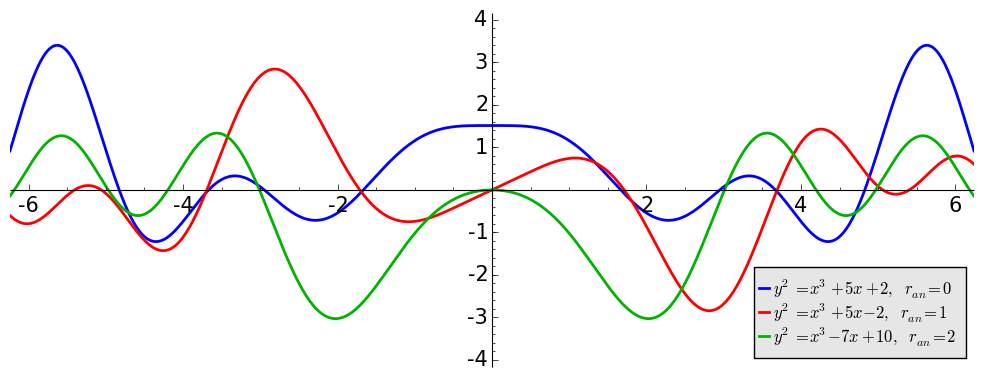
\includegraphics[width=1.0\textwidth]{graphics/L-functions_at_origin.png}
    \caption{The values of three elliptic curve $L$-functions along the critical line $1+it$ for $-6 \le t \le 6$, (transformed so that the functions are purely real to make the visualization a bit easier). Blue corresponds to a rank 0 curve, red is that of a rank 1 curve, and green is a rank 2 curve. Note that close to the origin the graphs look like non-zero constant function, a straight line and a parabola respectively.}
    \label{fig:L-functions_at_origin}
\end{figure}

We can therefore at least conjecturally determine the curve's algebraic rank by computing the order of vanishing of the elliptic curve's $L$-function at the central point. This converts an generally difficult algebraic problem into a perhaps more tractable analytic one.

The work in this thesis hopes to address the question of how to effectively compute the order of vanishing of $L(E,s)$ at $s=1$, which is denoted $r_{an}$, the {\it analytic rank} of $E$. This, again, is a non-trivial task -- for example, how do you numerically distinguish between the $n$th Taylor coefficient of $L(E,s)$ being identically zero, and it just being non-zero but so small in magnitude that it is indistinguishable from zero given your finite-precision computations?

The short answer is that, using a just a computer, you can't. We need theorems governing the magnitude of the Taylor coefficients -- especially that leading coefficient $C$ mentioned above -- in order to make analytic rank explicitly computable. This work establishes those results (assuming standard conjectures), telling us precisely how many digits of precision we need for an elliptic curve $L$-function to ascertain whether a given Taylor coefficient is or isn't zero. This in turn allows us to detail an algorithm to compute a curve's analytic rank with provable asymptotic time complexity . And thanks to the BSD conjecture, we therefore have a way to -- at least conjecturally -- compute the algebraic rank of $E$ with a concrete handle on how long the computation will take. \\

The phrases ``explicitly computable" and ``provable asymptotic time complexity" are given precise definitions in the main body of this thesis, so read on for a more formal statement of the main problem and results. \\

The structure of this dissertation is as follows: Chapter 2 more formally lays out the problem tackled in this work and quotes the major results obtained in this work. Chapter 3 consists of an exposition of the mathematical background relevant to this thesis; while chapter 4 contains proofs of the main results. Chapter 5 consists of analytic methods and results that allow one, for example, to obtain estimates on analytic rank when evaluating a curve's $L$-function directly is computationally infeasible. Chapter 6 consists of remarks and ideas for future work. Supporting computational evidence is supplied where relevant, as opposed to being collected in its own chapter. 